\section{Software Solution}
\label{s:system}

\subsection{Architecture Evolution}
\label{ss:arch}

Figure~\ref{fig:arch} shows the Phase~2 architecture. The Phase~1 design already planned a web UI calling a FastAPI backend that runs the pipeline; Phase~2 built it. Four things changed relative to the Phase~1 plan. (1) The REST interface became a single resource, \texttt{/api/recommendations}, created with \texttt{POST} and polled with \texttt{GET}, instead of separate \texttt{/recommend} and \texttt{/jobs/\{id\}} endpoints. (2) Jobs are stored in SQLite instead of an in-memory cache. (3) Stage~1 uses prompt v2 (Section~\ref{ss:stage1method}). (4) The verifier is fine-tuned (Section~\ref{ss:verifiermethod}). Two planned components were \emph{not} built and remain future work: a rule engine with the OSADL compatibility matrix, and vector retrieval, which is still replaced by deterministic clause selection because full license texts exceed the free tier's per-minute token limit.

A run takes 30\,s to 5\,min on the free tier, too long for one HTTP request. \texttt{POST} therefore validates the input and returns \texttt{202} with a job identifier at once; one worker thread runs jobs in order, because Groq's per-minute limit and the single verifier in memory make parallel runs slower, not faster. The UI polls every 1.5\,s and shows the current step and queue position.

\begin{figure*}[tb]
    \centering
    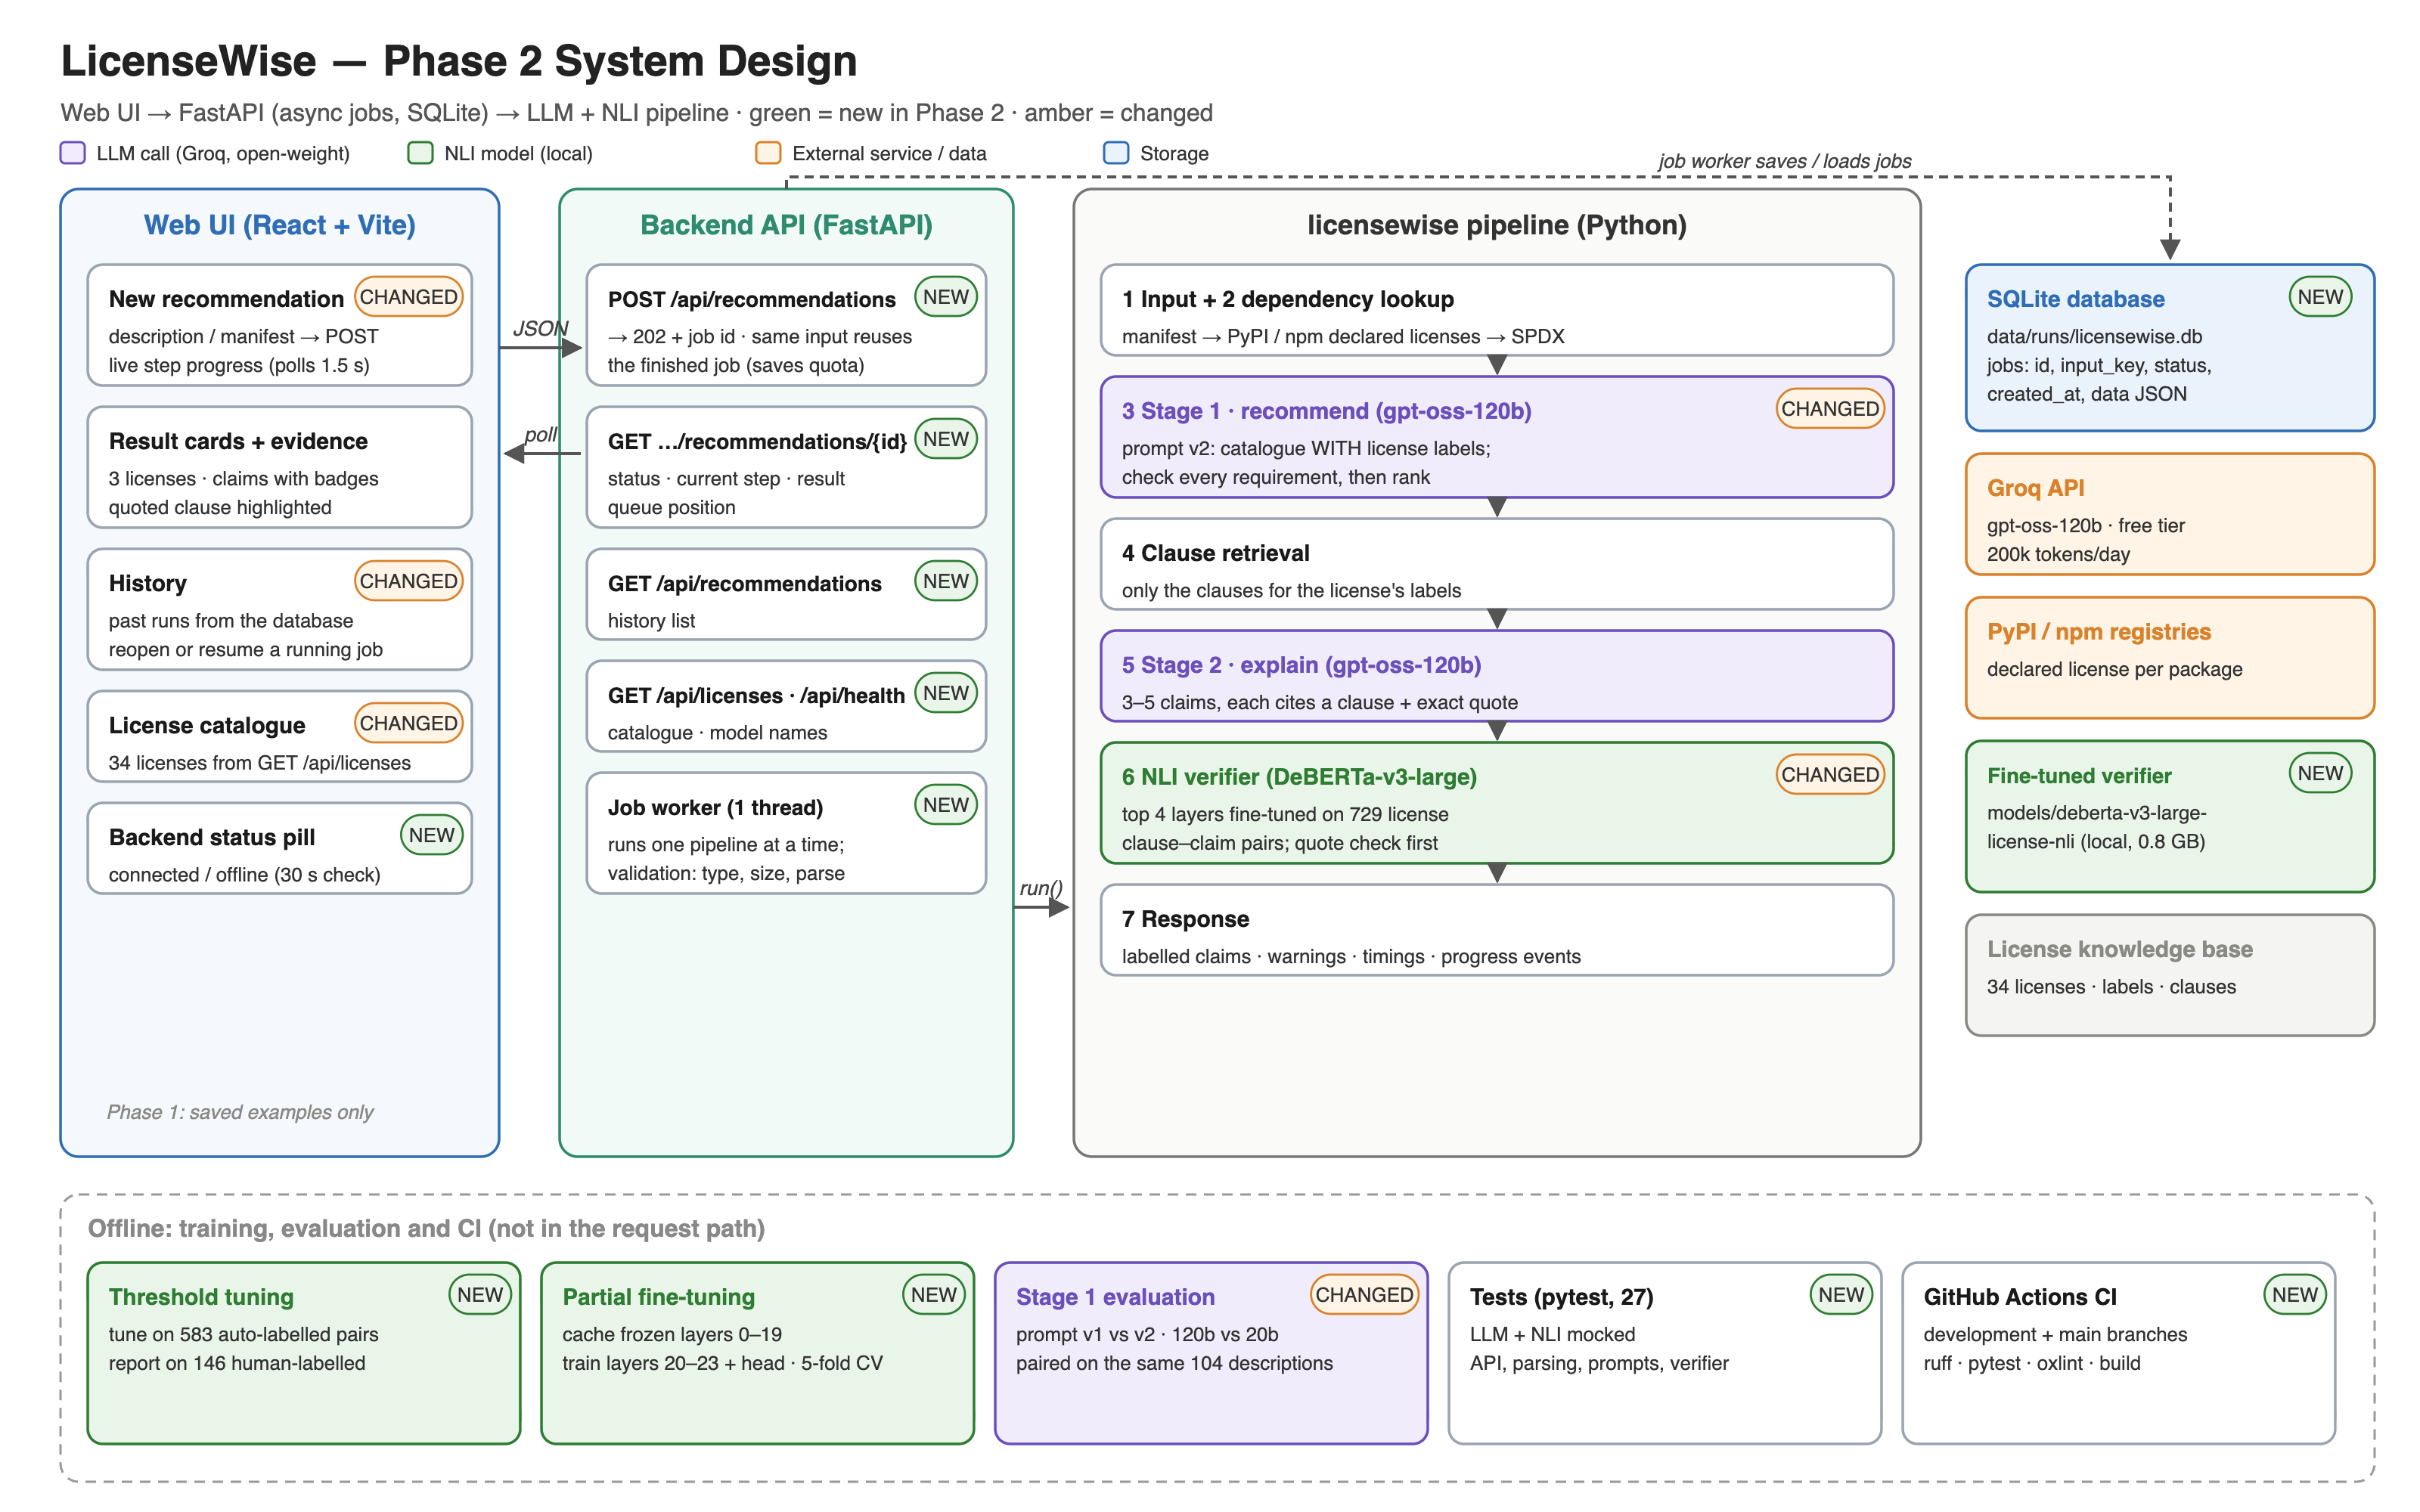
\includegraphics[width=0.94\textwidth]{p2_07_system_design_v2.png}
    \caption{Phase 2 system design. Green tags mark components new in Phase~2 and amber tags components changed since Phase~1. The offline strip holds training, evaluation, and CI, which are not in the request path.}
    \label{fig:arch}
\end{figure*}

\subsection{Implementation}
\label{ss:impl}

Table~\ref{tab:impl} lists the technology stack. The code is in the GitHub repository \texttt{AJFX-01/softwarelincense}. The pipeline is a Python package, \texttt{licensewise}, with one module per step; every LLM call requests output that conforms to a Pydantic JSON schema, and the Stage~1 schema restricts identifiers to the 34 catalogue entries. Input is validated before any LLM call: a description or a manifest is required, descriptions are capped at 4{,}000 characters, and manifests must be \texttt{requirements.txt}, \texttt{pyproject.toml}, or \texttt{package.json}, at most 100\,KB, parse correctly, and list dependencies. Invalid input returns HTTP 422. Rate-limit and missing-key errors are reported in plain language. If a request exceeds the free tier's per-minute token limit (HTTP 413), it is retried once with a smaller output cap.

\begin{table}[tb]
    \caption{Implementation stack.}
    \label{tab:impl}
    \centering
    \footnotesize
    \begin{tabularx}{\columnwidth}{@{}lX@{}}
        \toprule
        \textbf{Layer} & \textbf{Technology} \\
        \midrule
        Front end & React 19, TypeScript, Vite; pages for new recommendation, history, and licenses \\
        Backend & FastAPI + Uvicorn (Python 3.14); 5 endpoints; 1 worker thread \\
        Database & SQLite (Python standard library) \\
        LLM & gpt-oss-120b via Groq, JSON-schema output (Stages 1 and 2) \\
        Verifier & DeBERTa-v3-large NLI, top 4 of 24 layers fine-tuned (PyTorch, Transformers, Apple MPS); runs locally, 0.8\,GB \\
        Data & choosealicense.com, SPDX, Software Heritage, PyPI, npm \\
        Quality & pytest (27 tests), ruff, oxlint, \texttt{tsc} \\
        CI/CD & GitHub Actions; branches \texttt{development} and \texttt{main} \\
        \bottomrule
    \end{tabularx}
\end{table}

\subsection{Database}
\label{ss:db}

Jobs are stored in a single SQLite table, \texttt{jobs(id, input\_key, status, created\_at, data)}, indexed on \texttt{created\_at}. SQLite suits a single-user tool: it needs no server, writes are atomic (a crash cannot leave a half-written record, which happened with the Phase~1 JSON files), and history can be queried by status and time. \texttt{input\_key} is a SHA-256 hash of the model, description, manifest, and verification flag; an identical request reuses the finished result instead of spending LLM quota again. \texttt{data} holds the full nested pipeline result as JSON because its shape is still evolving. On startup, jobs left queued or running by a restart are marked failed with a clear message, and Phase~1 job files are imported once.

\subsection{UI and Backend Integration}
\label{ss:ui}

The UI calls \texttt{GET /api/health} every 30\,s to show a ``backend connected/offline'' indicator; \texttt{POST /api/recommendations} starts a run (or reuses an identical one); \texttt{GET /api/recommendations/\{id\}} reports the live step (dependency lookup, Stage~1, retrieval, explanation, verification); \texttt{GET /api/recommendations} lists history; and \texttt{GET /api/licenses} serves the catalogue with labels and copyleft level. Figure~\ref{fig:ui} shows the user flow: enter a description or manifest, follow the run, read three license cards whose claims carry status badges, and open the cited clause with the quoted words highlighted and the NLI probabilities. Badges combine an icon with a text label, so status is never conveyed by colour alone.

\begin{figure}[tb]
    \centering
    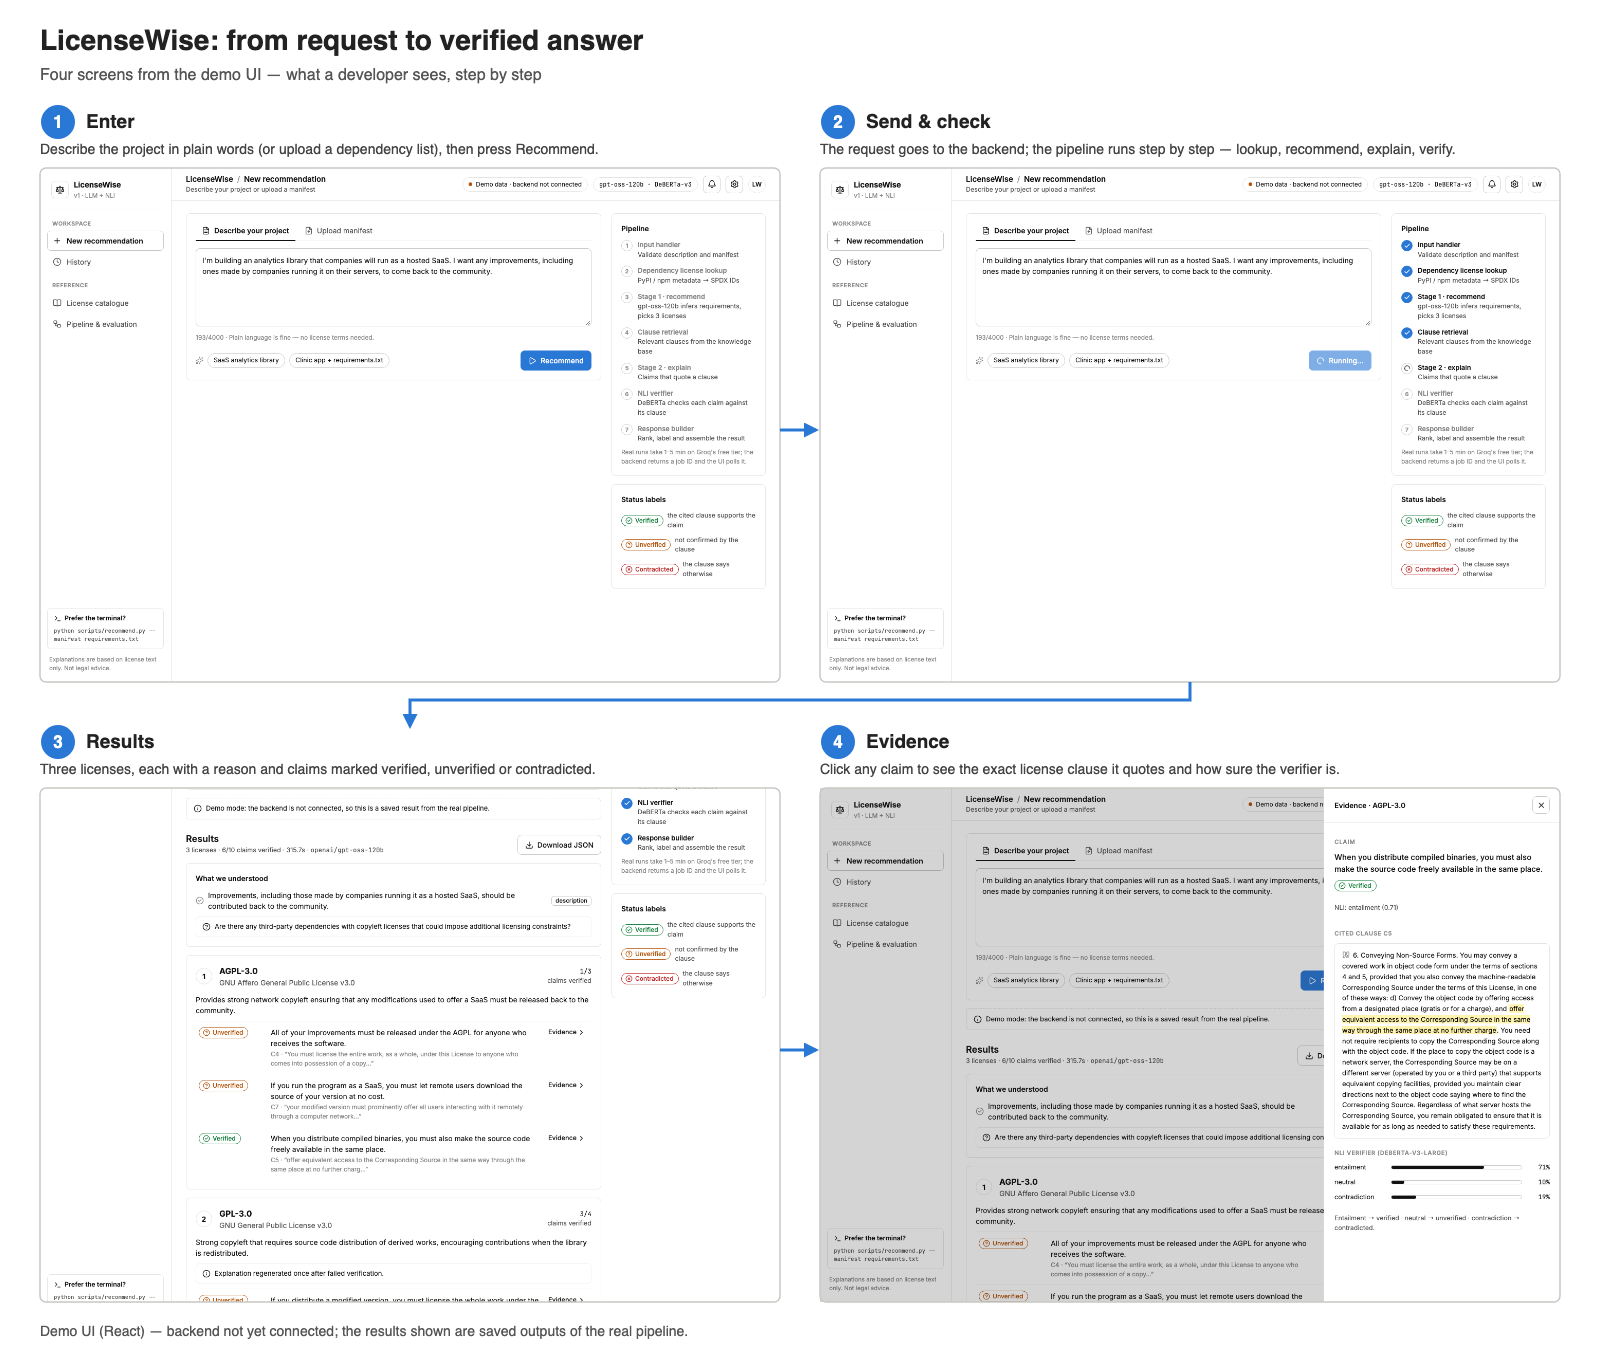
\includegraphics[width=\columnwidth]{22_ui_storyboard.png}
    \caption{User flow: (1) input, (2) live pipeline steps, (3) results with verified/unverified/contradicted claims, (4) evidence with the highlighted clause.}
    \label{fig:ui}
\end{figure}

\subsection{CI/CD and GitHub Integration}
\label{ss:ci}

Figure~\ref{fig:ci} shows the workflow. Work lands on \texttt{development}; \texttt{main} is the stable, demo-ready branch and changes only through a pull request whose checks pass. GitHub Actions runs on every push and pull request to either branch, with two jobs. The \emph{backend} job installs a CI requirements file and runs \texttt{ruff} and \texttt{pytest}. The \emph{ui} job installs dependencies with a frozen lockfile and runs \texttt{oxlint}, the TypeScript type-check, and the Vite build, so the UI that talks to the API is checked on every change. The 27 tests replace the LLM and NLI calls with fakes and use a temporary database, so CI needs no API key or model, installs no PyTorch, and runs the suite in under a second. The tests cover the API contract (202 and polling, reuse, 422/404 errors, persistence across restarts), manifest parsing, license normalisation, the Stage~1 prompt variants and retry logic, and the verifier's quote check. They also found a real defect: the worker pool was created at import time, so the application could not restart within one process; it is now created in the FastAPI lifespan handler.

\begin{figure*}[tb]
    \centering
    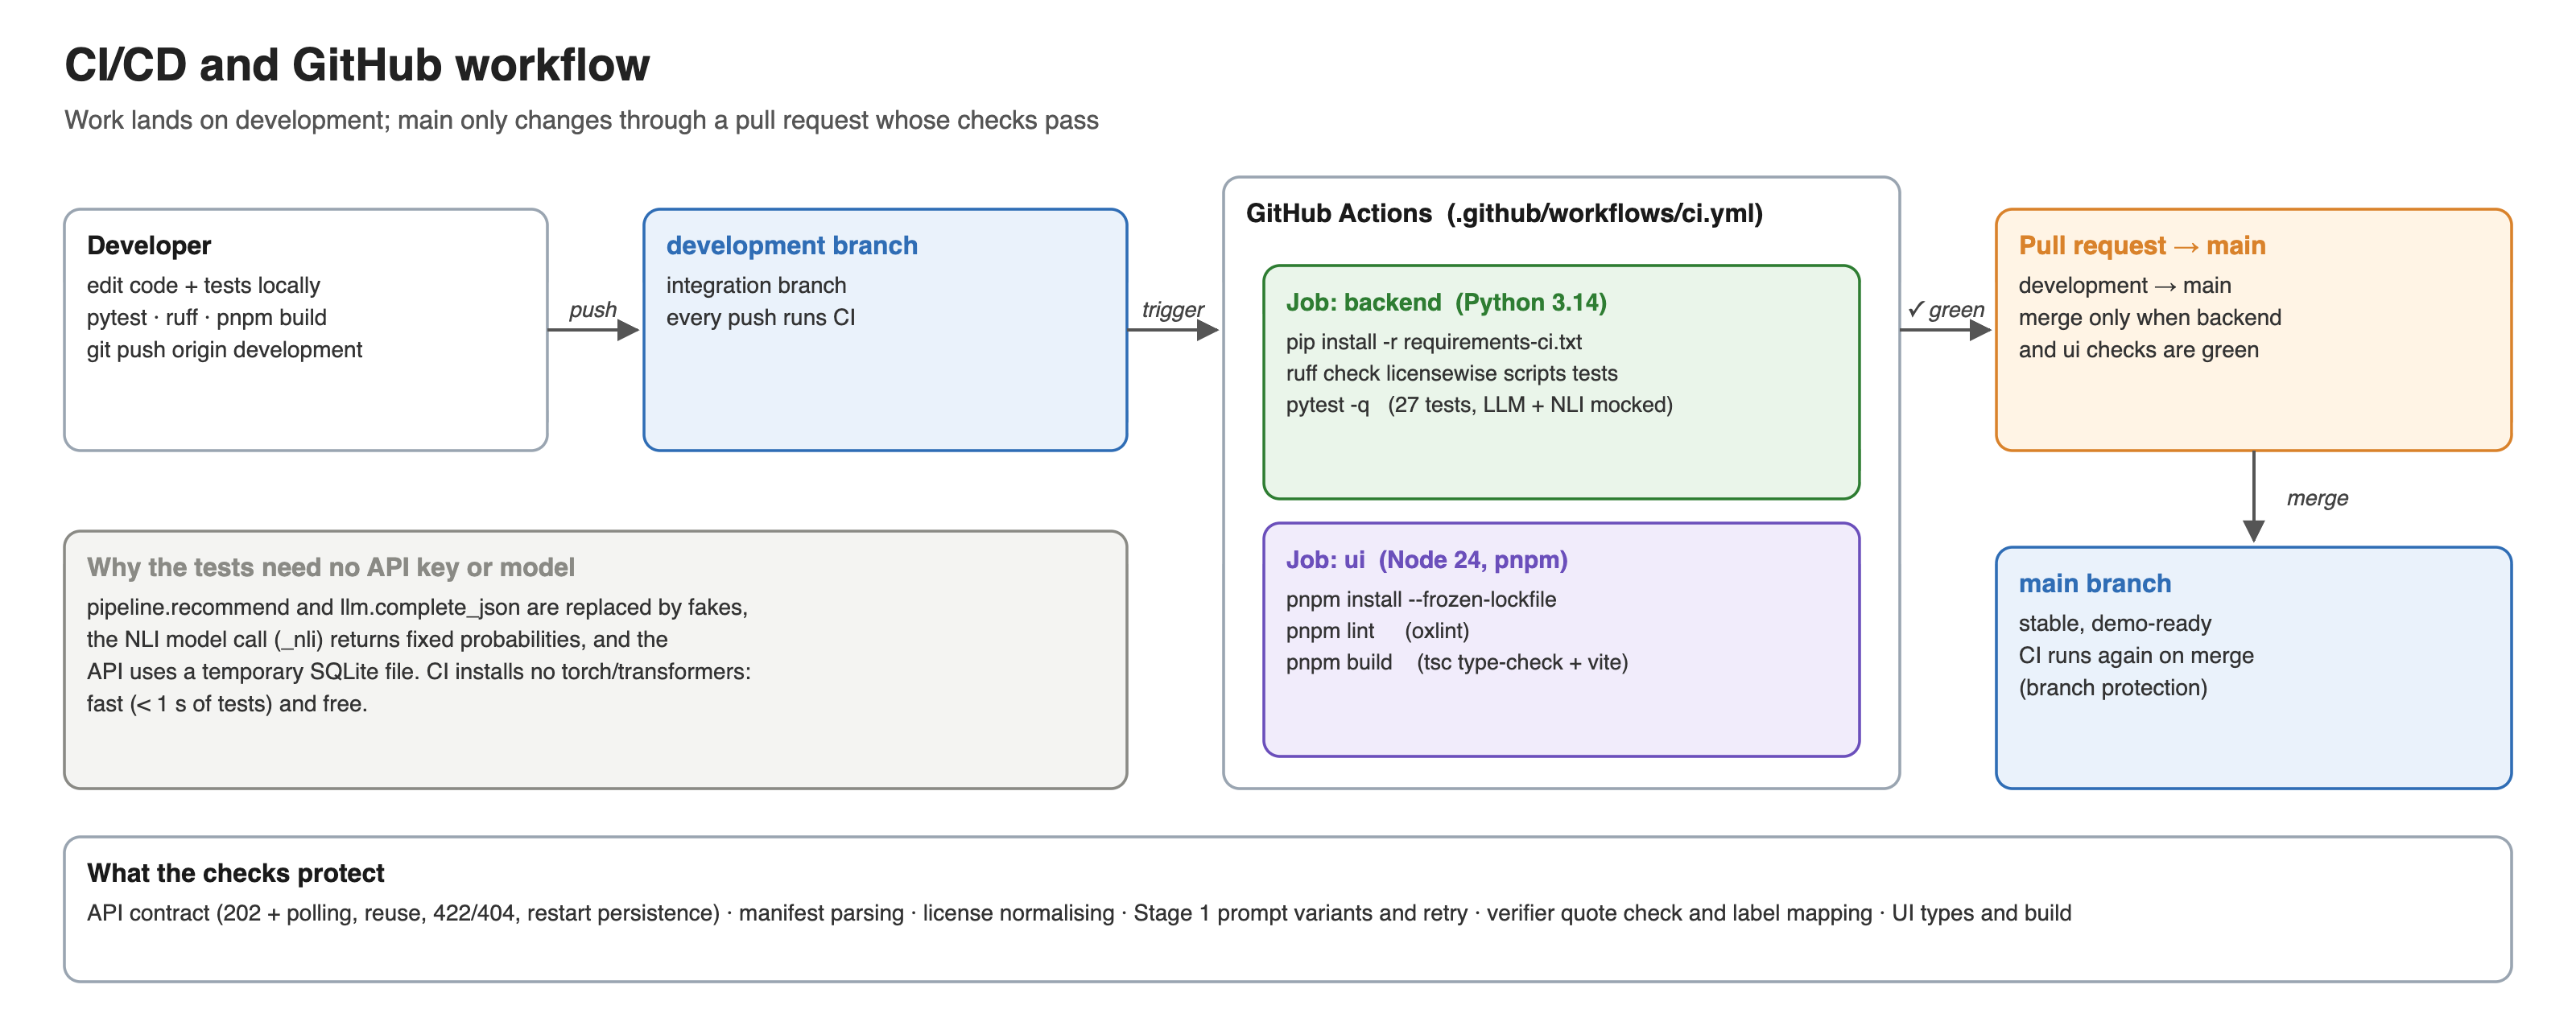
\includegraphics[width=0.85\textwidth]{p2_08_cicd.png}
    \caption{CI/CD workflow: pushes to \texttt{development} trigger the backend and UI jobs; \texttt{main} changes only through a pull request with passing checks.}
    \label{fig:ci}
\end{figure*}
